\documentclass{article}
\usepackage{graphicx} % Required for inserting images
\usepackage{amsmath}
\usepackage{hyperref} % https://www.overleaf.com/learn/latex/Hyperlinks
\usepackage{CJKutf8} % https://www.overleaf.com/learn/latex/Chinese
\usepackage{biblatex} % https://www.overleaf.com/learn/latex/Bibliography_management_with_biblatex
\addbibresource{reference.bib}

\title{11220CS515400 Hardware Security\\Programming Assignment 3 Report}
\author{109062319 \begin{CJK*}{UTF8}{bkai}楊智明\end{CJK*}}
\date{June 11, 2024}

\begin{document}

\maketitle

\section{How To Use The VCS Tool}

\subsection{Setting Up The Environment}

According to the document of PA3, we should first set up the environment for VCS and Verdi with the following \verb|source| commands:

\begin{verbatim}
[ts109062319@cad ~]$ source /usr/cad/synopsys/CIC/vcs.cshrc
[ts109062319@cad ~]$ source /usr/cad/synopsys/CIC/verdi.cshrc
\end{verbatim}

\subsection{Compilation}

To learn how to use VCS, it helps to simply type in \verb|vcs| in the command line first:

\begin{verbatim}
[ts109062319@cad ~]$ vcs
VCS MX compilation command help:
   (1) Unified use model for all design topologies :
       vcs [libname.]<Top Module_Or_Entity_Or_Config> [compile op
ts]

   (2) Two step use model for pure verilog design only :
       vcs <source_files> [compile opts]

   where frequently used [compile opts] are,
      [-debug][-debug_access+all][-o <log_file_name>][+rad][-cm][
-sdf][-P <pli tab>]

   For more information,
       About the use model (1), Please refer chapter [4] in VCS M
X User Guide or
       About the use model (2), Please refer chapter [3] in VCS U
ser Guide or
       Type vcs -help
\end{verbatim}

According to the message shown in the previous page, \verb|vcs <source_files>|\\\verb|[compile opts]| would be the command I use to invoke VCS. \verb|<source_files>| is simply all the \verb|.v| files; if VCS supports wildcard expansion, I can simply write \verb|*.v|. For \verb|[compile opts]|, according to \cite{csdnverdicov}, I at least need the \verb|-cm| switch in order to enable code coverage.

\begin{verbatim}
[ts109062319@cad ~]$ vcs *.v -cm line+cond+tgl+fsm+branch
*** Using c compiler gcc instead of cc ...
/usr/cad/synopsys/vcs/cur/linux/bin/vcs1: error while loading sha
red libraries: libelf.so.1: cannot open shared object file: No su
ch file or directory
CPU time: .023 seconds to compile
\end{verbatim}

It does not work yet. According to eeclass discussion, I should also specify \verb|-full64| when using VCS. To learn what this option exactly does, I can type in \verb|vcs -help| and then \verb|/-full64<ENTER>| to go to this option.

\begin{verbatim}
-full64
   Compiles the design in 64 bit mode and creates a 64 bit
   executable for simulating in 64 bit mode.
\end{verbatim}

It looks like the workstation is in 64 bit only mode, but the default mode in VCS is 32 bit. In fact, I even searched for all the accessible \verb|libelf.so.1|s:

\begin{verbatim}
[ts109062319@cad ~]$ find / -name libelf.so.1 > ~/libelf.txt
...
find: ...: Permission denied
...
[ts109062319@cad ~]$ cat libelf.txt
/home/tools/INCISIV/INCISIVE_15.20.039/tools.lnx86/lib/64bit/SuSE
/libelf.so.1
/home/tools/INCISIV/INCISIVE_15.20.039/tools.lnx86/lib/SuSE/libel
f.so.1
/home/tools/INNOVUS/INNOVUS18.11/tools.lnx86/lib/SuSE/libelf.so.1
/home/tools/INNOVUS/INNOVUS18.11/tools.lnx86/lib/64bit/SuSE/libel
f.so.1
/home/tools/IC/IC51.41.151/tools.lnx86/lib/64bit/SuSE/libelf.so.1
/home/tools/IC/IC51.41.151/tools.lnx86/lib/SuSE/libelf.so.1
/usr/lib64/libelf.so.1
\end{verbatim}

According to the search result shown above, some other tools on the workstation have their own \verb|libelf.so.1| in both 32 bit mode and 64 bit mode, but VCS does not, and thus it resorts to the default \verb|libelf.so.1| in 32 bit mode, which I believe would be located at \verb|/usr/lib/libelf.so.1| and, unfortunately, does not exist. This gives a complete reason that the option \verb|-full64| is required on this specific VCS workstation.

\begin{verbatim}
[ts109062319@cad ~]$ vcs *.v -cm line+cond+tgl+fsm+branch -full64
*** Using c compiler gcc instead of cc ...
                      Chronologic VCS (TM)
      Version P-2019.06_Full64 -- Mon Jun 10 13:34:46 2024
            Copyright (c) 1991-2019 by Synopsys Inc.
                      ALL RIGHTS RESERVED

This program is proprietary and confidential information of
Synopsys Inc. and may be used and disclosed only as authorized in
a license agreement controlling such use and disclosure.

Parsing design file 'aes_128.v'
Parsing design file 'aes_top.v'

Error-[ITSFM] Illegal `timescale for module
aes_top.v, 20
  Module "aes_top" has `timescale but previous module(s)/package(
s) do not.
  Please refer LRM 1364-2001 section 19.8.
...
\end{verbatim}

It still does not work, but this time the error message is readable. It basically says that \verb|aes_top.v| has \verb|`timescale| but \verb|aes_128.v| (the only \textit{previous module file}) does not. Obviously, one way to fix the problem is to disallow wildcard expansion and specify the order of the source files by myself. Now the following command correctly compiles my Verilog files.

\begin{verbatim}
[ts109062319@cad ~]$ vcs aes_top.v aes_128.v round.v table.v tb.v
 -cm line+cond+tgl+fsm+branch -full64
\end{verbatim}

\subsection{Simulation (The Wrong Version)}

According to \cite{ytverdiprep}, the compilation step generates an executable named \verb|simv|, and to run the simulation, all I need is to execute this file directly.

\begin{verbatim}
[ts109062319@cad ~]$ ./simv
\end{verbatim}

However, this is currently incorrect, and the error can not be detected here. I shall identify and fix it later.

\subsection{Visualization Using Verdi Coverage}

\begin{verbatim}
[ts109062319@cad ~]$ ls
aes_128.v  cm.log  Makefile  simv         simv.vdb  tb.v
aes_top.v  csrc    round.v   simv.daidir  table.v   ucli.key
[ts109062319@cad ~]$ verdi -cov -covdir simv.vdb
\end{verbatim}

According to \cite{ytverdicov}, the previous command opens the specified coverage\\database, which is a \verb|.vdb| folder, in Verdi Coverage.

\begin{figure}[t] \centering
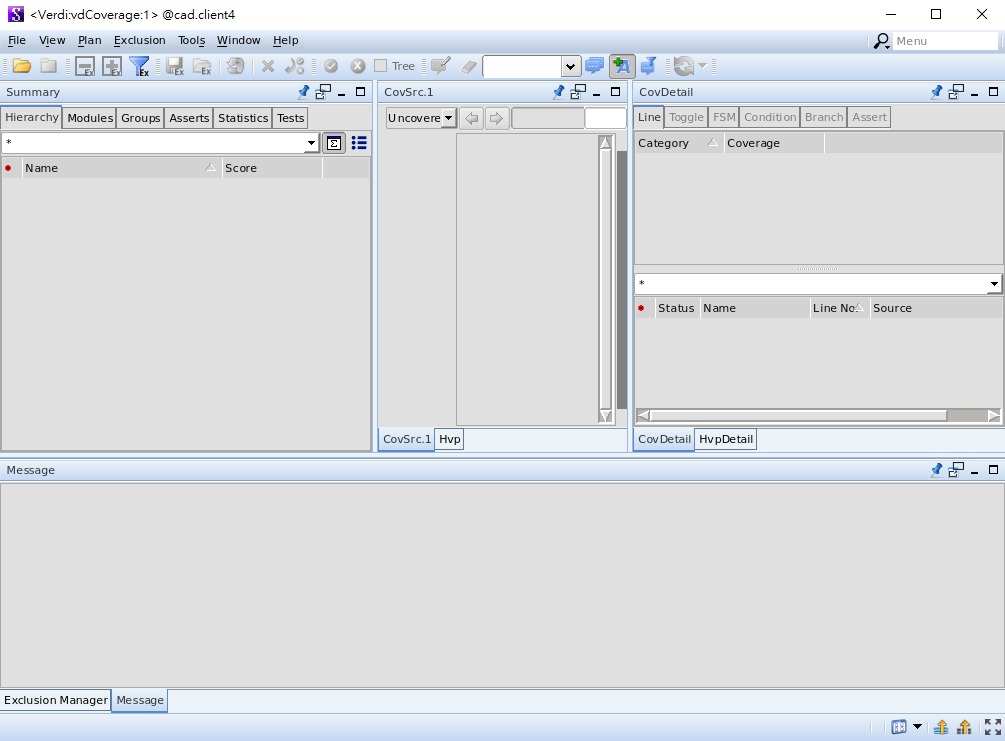
\includegraphics[width=0.666667\textwidth]{simv_no_cm}
\caption{The Verdi Coverage report after running \texttt{./simv} and \texttt{verdi -cov -covdir simv.vdb}.}
\label{simv_no_cm}
\end{figure}

\subsection{Simulation (The Correct Version)}

The coverage report does not show up in Figure \ref{simv_no_cm}. What could go wrong with those commands? I believe all of my references are \textit{trusted}?

Later I randomly came across Figure \ref{A Quick Start Example}. Maybe this can help me out?

\begin{figure}[h] \centering
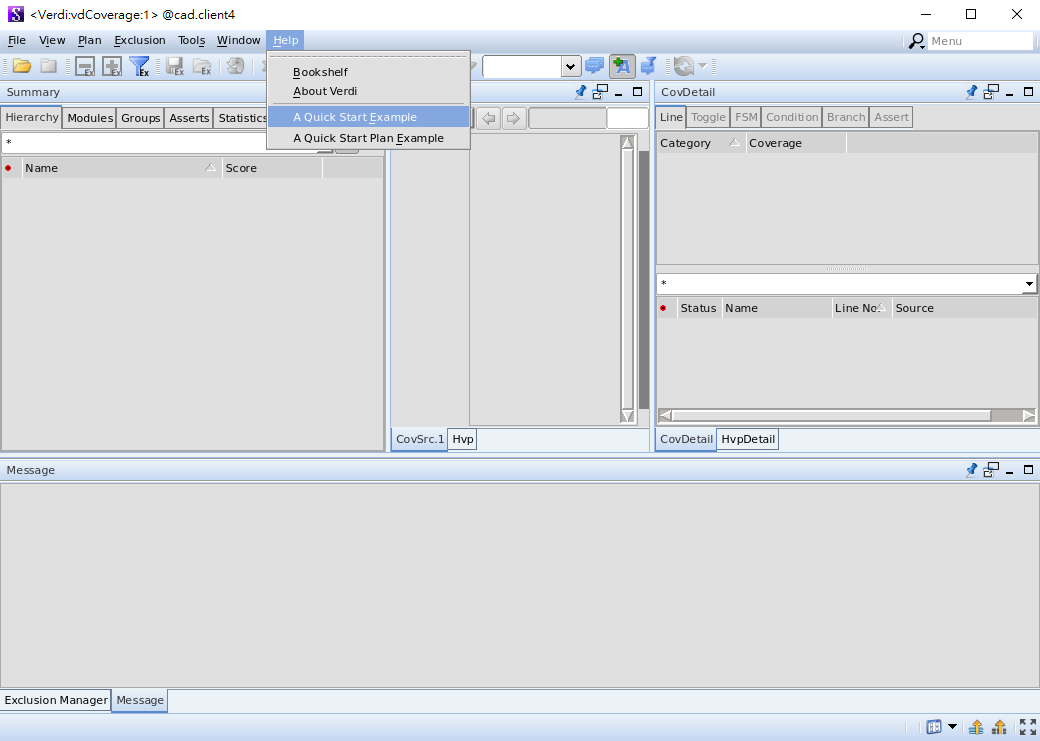
\includegraphics[width=0.666667\textwidth]{A Quick Start Example}
\caption{A Quick Start Example in Verdi Coverage.}
\label{A Quick Start Example}
\end{figure}

I clicked the button and nothing happened. I closed Verdi and realized that something did happen. I traced the example codes and found the error, which can be seen in the next page.

\begin{verbatim}

[ts109062319@cad ~]$ grep -d skip simv *
...
tr690.csh:simv -cm line+tgl+cond+fsm
...
\end{verbatim}

It means that, when simulating, I need to pass the \verb|-cm| option to the \verb|simv| executable as well. Giving this option to VCS means that VCS would compile the code for the specified coverages, but it does not imply that the simulation would be run with the same set of coverages.

As a result, the correct simulation command is shown below.

\begin{verbatim}
[ts109062319@cad ~]$ ./simv -cm line+cond+tgl+fsm+branch
\end{verbatim}

\subsection{How To Execute The Makefiles \cite{gnumake}}

As stated in the PA specification, type \verb|make com| to compile the Verilog files into the simulation executable, type \verb|make sim| to run the actual simulation, and type \verb|make cov| to show the code coverage in Verdi Coverage. Additionally, in my makefile, simply typing \verb|make| is the same as compiling, i.e. \verb|make com|.

My makefiles also supports rebuilding from scratch. Type \verb|make clean| to remove all the file related to compilation. Note that my \verb|make clean| does not remove logs such as \verb|cm.log| and \verb|vdCovLog/| and it does not remove \verb|novas.conf| and \verb|novas.rc|.

\section{Code Coverage Of The Sample Code}

\begin{figure}[h] \centering
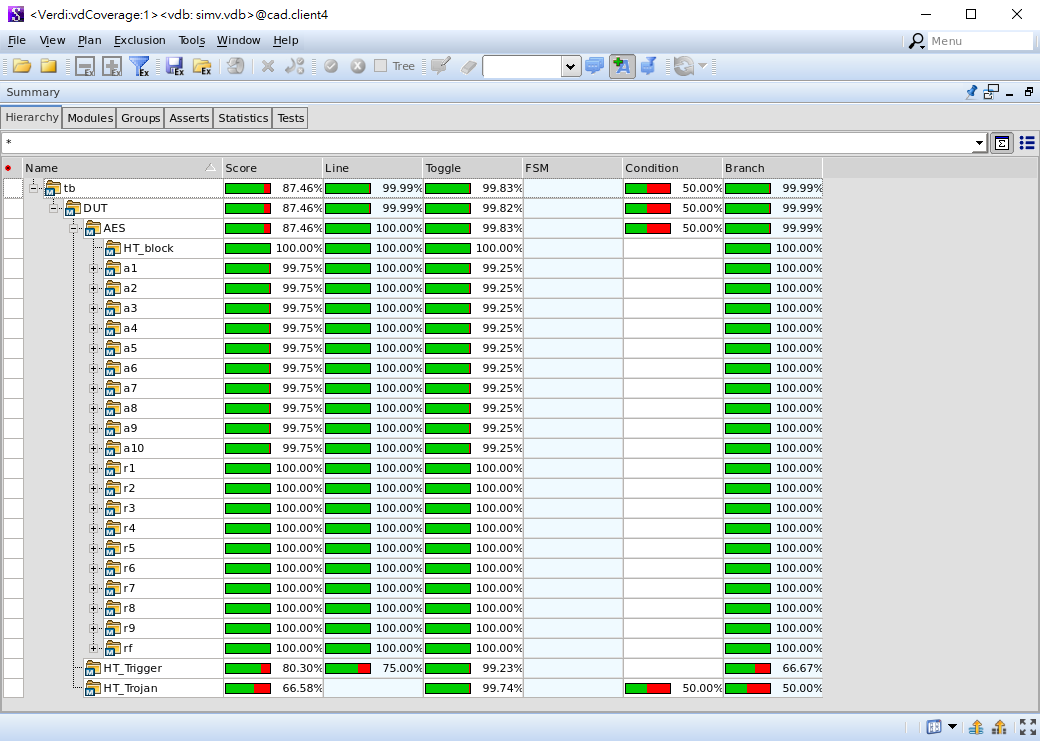
\includegraphics[width=0.8\textwidth]{HT}
\caption{The code coverage of the sample code in Verdi Coverage.}
\label{HT}
\end{figure}

\section{Identifying The Three Hardware Trojans}

\subsection{HT1}

The condition coverage of \verb|HT_Trojan| is suspicious. Let's dive in and check what the uncovered condition(s) are:

\begin{figure}[h] \centering
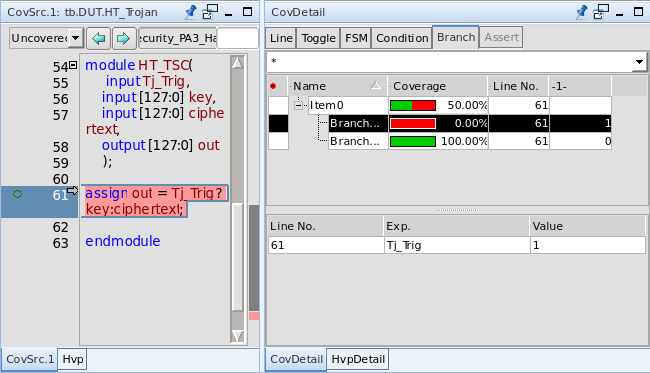
\includegraphics[width=0.75\textwidth]{HT1-1}
\caption{The \textit{branch} coverage of \texttt{HT\_Trojan}. Note that in this case, the branch coverage conveys the same message as the condition coverage.}
\label{HT1-1}
\end{figure}

In Figure \ref{HT1-1}, the branch 1 is never taken during the simulation. In other cases, \verb|out| is always equal to \verb|ciphertext|. By the UCI \cite{5504712} method, \verb|out| should be directly assigned to \verb|ciphertext|. After cleaning up the code further, the code coverage of \verb|HT1/nHT| is shown in Figure \ref{nHT1}.

\begin{figure}[h] \centering
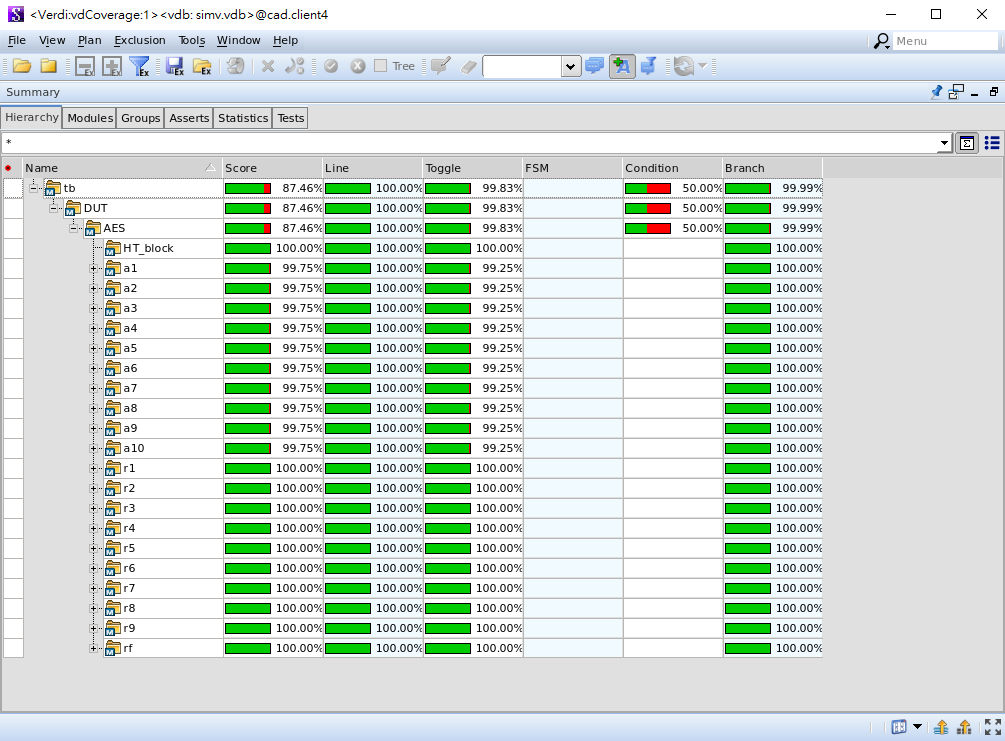
\includegraphics[width=0.75\textwidth]{nHT1}
\caption{The code coverage of \texttt{HT1/nHT}.}
\label{nHT1}
\end{figure}

It looks like the code coverage was not much different from Figure \ref{HT}. This is because the number of lines, conditions and branches affected by HT1 is much smaller than the total number of them, and that I eventually removed the two HT1-related modules altogether.

\begin{figure}[t] \centering
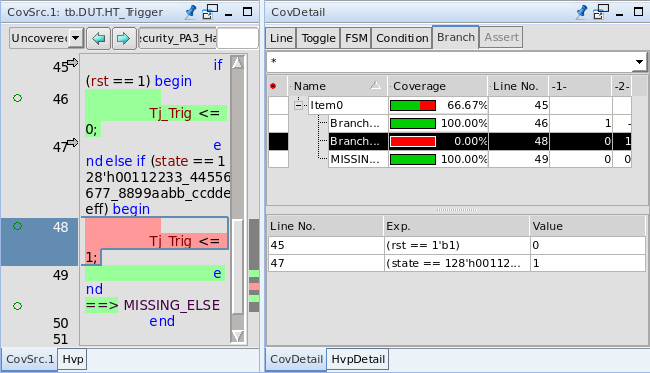
\includegraphics[width=\textwidth]{HT1-2}
\caption{The trigger of HT1.}
\label{HT1-2}
\end{figure}

The payload of this hardware Trojan can be inferred from Figure \ref{HT1-1}: replacing the ciphertext, the result of AES-128 encryption, with the key. The trigger of this hardware Trojan is located somewhere else, in the module \verb|HT_Tri| in Figure \ref{HT1-2}. Basically, the hardware Trojan is triggered when the input state (plaintext) equals a specific value.

However, the trigger is more than this: since there is a missing \verb|else| in the RTL code, the trigger signal is latched once enabled, and the hardware Trojan remains on until it is reset. A circuit representation of \verb|HT_Tri| is shown in Figure \ref{HT_Tri}.

\begin{figure}[h] \centering
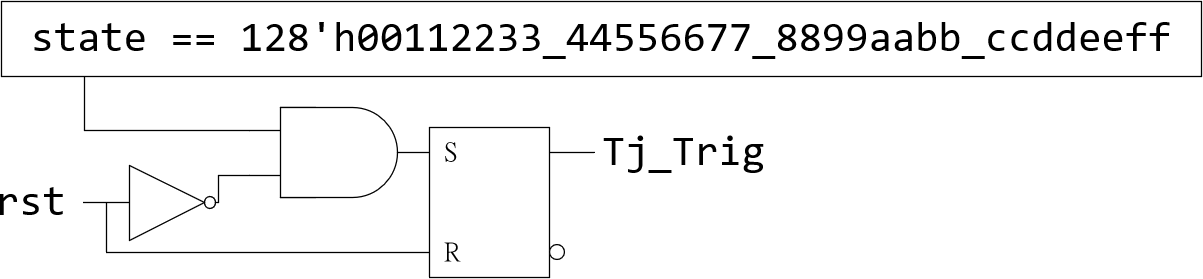
\includegraphics[width=\textwidth]{HT_Tri}
\caption{The trigger condition of HT1, with an explicit latch.}
\label{HT_Tri}
\end{figure}

\subsection{HT2}

Another suspicious part is the condition coverage of \verb|AES|. The uncovered condition is shown in Figure \ref{HT2-1}. Again, the branch 1 is never taken during the simulation. By the UCI method again, \verb|out| should be directly assigned to \verb|HT_normal_out|.

\begin{figure}[htp] \centering
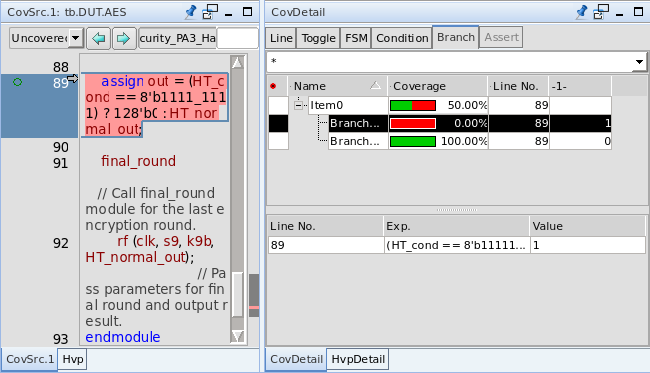
\includegraphics[width=0.85\textwidth]{HT2-1}
\caption{The uncovered branch of \texttt{AES}.}
\label{HT2-1}
\end{figure}

Now, where does \verb|HT_cond| come from? It consists of 9 bits, each of which comes from each of the first 9 rounds. Interestingly, these 9 bits are triggered individally with full coverage during the simulation, as can be seen in Figure \ref{HT2-2}.

\begin{figure}[htp] \centering
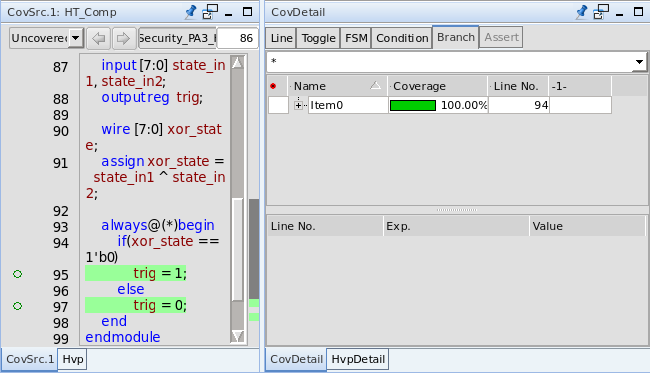
\includegraphics[width=0.85\textwidth]{HT2-2}
\caption{The triggering signal in \texttt{HT\_Comp}.}
\label{HT2-2}
\end{figure}

Now we can analyze the trigger and payload of HT2. As can be seen in Figure \ref{HT2-2}, each bit of \verb|HT_cond| is asserted when \verb|xor_state == 1'b0|, or \verb|state_in1 == state_in2|. Since the module in Figure \ref{HT2-2} is only instantiated in Figure \ref{HT2-3}, what it eventually does is comparing whether the \textbf{least significant byte} of the input state and the output state of \verb|one_round| is equal at a moment. (Note that the output is delayed by two clock cycles.) Finally, the trigger condition of HT2 is whether the least significant byte of \verb|s0| to \verb|s8| are all equal, \textbf{but not equal between} \verb|s8| \textbf{and} \verb|s9| (because there are 9 bits in \verb|HT_cond| but only 8 in the RHS, \verb|8'b1111_1111|.)

\begin{figure}[htp] \centering
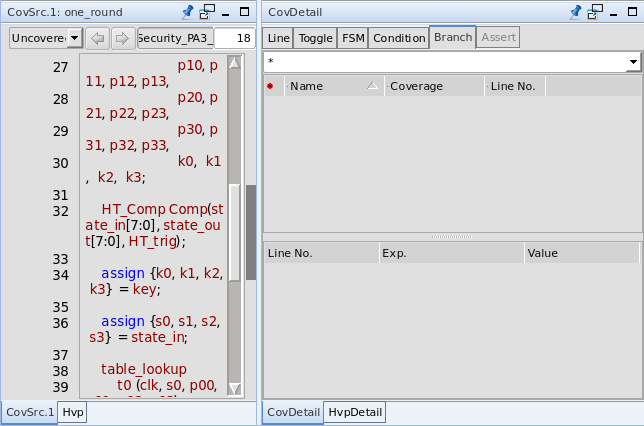
\includegraphics[width=0.666667\textwidth]{HT2-3}
\caption{The only instantiation of \texttt{HT\_Comp}.}
\label{HT2-3}
\end{figure}

The payload of HT2 is, again, shown in Figure \ref{HT2-1}: it simply replaces the output of AES-128 with zero.

\subsection{HT3}

\begin{figure}[htp] \centering
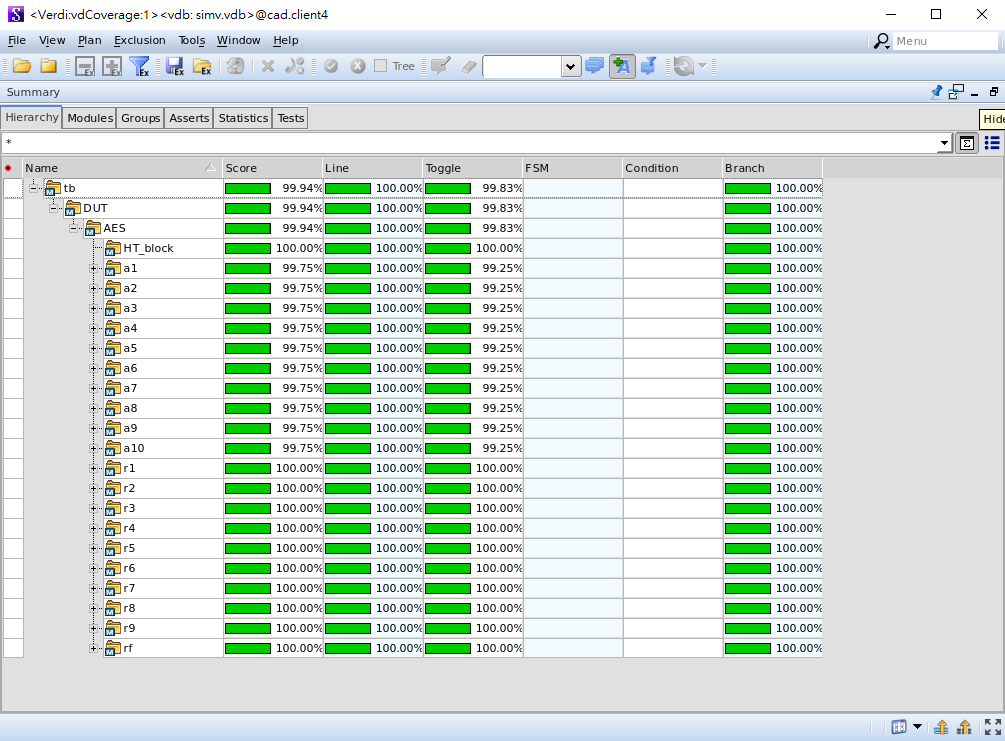
\includegraphics[width=0.666667\textwidth]{nHT12}
\caption{The code coverage with only HT3 present.}
\label{nHT12}
\end{figure}

The code coverage after removing \textit{both} HT1 and HT2 is shown in Figure \ref{nHT12}. The next thing to check might be the toggle coverage of \verb|a1| to \verb|a10|. However, this time the uncovered toggle does not correspond to a hardware Trojan. As can be seen in Figure \ref{rcon_toggle}, the signal \verb|rcon| is not toggled because it is meant to be a round \textit{constant}.

\begin{figure}[htp] \centering
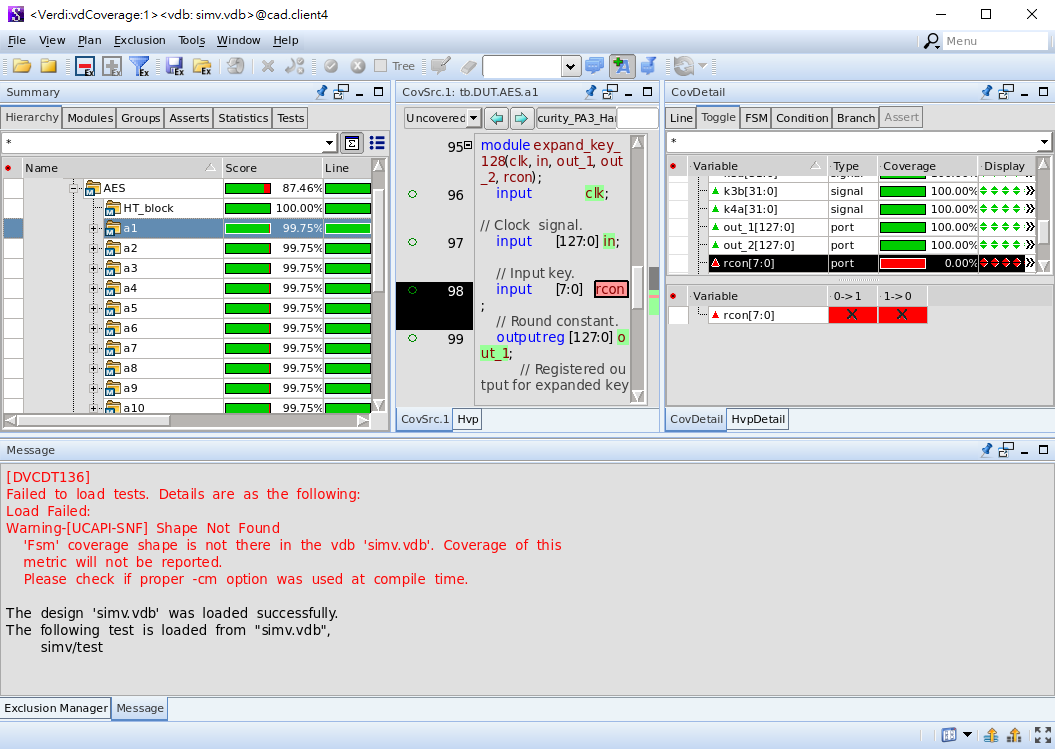
\includegraphics[width=0.96\textwidth]{rcon_toggle}
\caption{The toggle coverage does not cover \texttt{rcon}.}
\label{rcon_toggle}
\end{figure}

Interestingly, the actual Trojan is contained in \verb|HT_block|, and it has 100\% code coverage! In other words, this hardware Trojan can never be identified if we only analyzed the code coverage.

\begin{verbatim}
module HT_dynamic_key (clk, rst, key, HT_key);
    input [127:0] key;
    input clk, rst;
    output reg [127:0] HT_key;

    always@(posedge clk, posedge rst) begin
        if (rst)
            HT_key <= 128'd0;
        else if(HT_key == 128'd0)
            HT_key <= key;
        else
            HT_key <= 128'd0;
    end
endmodule
\end{verbatim}

The main module of HT3 is shown in the previous page. Basically, what it does is to leak the key into a register every 2 clock cycles (unless the key is exactly zero.) However, as I check where the module is instantiated, it is located somewhere shown below, and the signal \verb|HT_output| is not connected to anywhere else.

\begin{verbatim}
module aes_128(clk, rst, state, key, out);
...
    wire [127:0] HT_output;
    HT_dynamic_key HT_block(clk, rst, key, HT_output);
...
endmodule
\end{verbatim}

Therefore, this hardware Trojan does \textit{absolutely} nothing at the RTL, and I would classify HT3 as an \textit{always-on} Trojan which leaks the key via a possible \textit{side channel} every two clock cycles.

\section{Improving The Stealthiness Of The HTs}

For reference, Figure \ref{nHT123} is the code coverage without any hardware Trojan.

\begin{figure}[htp] \centering
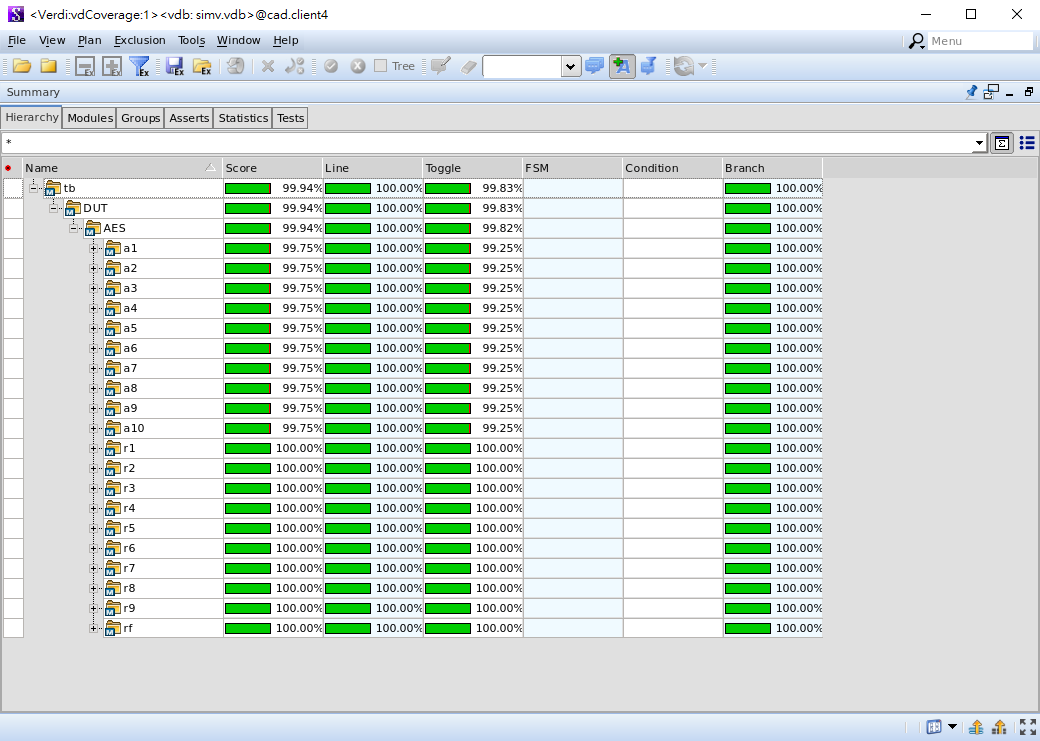
\includegraphics[width=\textwidth]{nHT123}
\caption{The code coverage without any hardware Trojan.}
\label{nHT123}
\end{figure}

\subsection{HT1}

My improvement of the stealthiness of HT1 is based on \cite{6581574}. In Section III-B of the paper, it is suggested that the trigger condition should be partitioned into \textit{sub-trigger conditions} and, assuming that the sub-trigger conditions are \verb|t[0]|, \verb|t[1]|, ..., and \verb|t[k-1]|, that the code related to the trigger and the payload of the HT should be written in this style, instead of conditional statements using, for example, the \verb|?:| operator:

\begin{verbatim}
always @(posedge clk) begin
    f <= (t[0] & t[1] & ... & t[k-1]) & f_m |
         (~t[0] | ~t[1] | ... | ~t[k-1]) & f_n;
end
\end{verbatim}

In my improvement of HT1, there are 16 sub-trigger conditions, each of which corresponds to one byte. Then, the sub-trigger conditions and the payload are integrated according to the suggested coding style. I leveraged the unary operators \verb|&| and \verb|~&| in Verilog as well so that the resulting code is less ugly (too ugly a piece of code can also draw attention to designers!) I also augmented the latch state to use 16 bits instead of 1, so that the latch state bits are actually toggled during simulation, and the improved HT1 has \textit{exactly} the same trigger and payload of the original HT1. The latch state bit(s) are also migrated from \verb|HT_Tri| to \verb|HT_TSC|. The resulting code coverage is shown in Figure \ref{improveHT1}.

\begin{figure}[htp] \centering
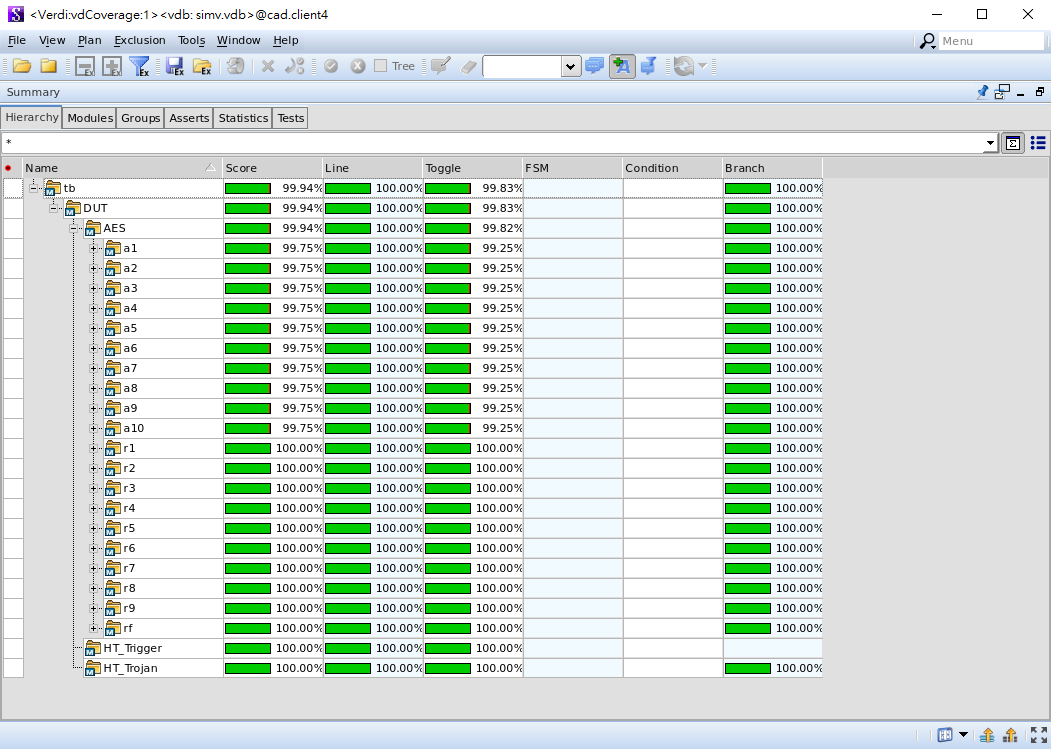
\includegraphics[width=\textwidth]{improveHT1}
\caption{The code coverage of \texttt{HT1/improveHT}.}
\label{improveHT1}
\end{figure}

\subsection{HT2}

My improvement of the stealthiness of HT1 is based on \cite{5958022}. Figure \ref{Product of sums attack} shows one of the proposed attacks, where $i_0$ and $i_1$ are non-trigger inputs and $t_0,t_1,\cdots,$\\$t_{n-1}$ are the trigger inputs. The trigger condition is $t_0\wedge t_1\wedge\cdots\wedge t_{n-1}$. Under non-trigger conditions the output $f$ is $i_0\wedge i_1$; under trigger conditions the output is 1.

\begin{figure}[htp] \centering
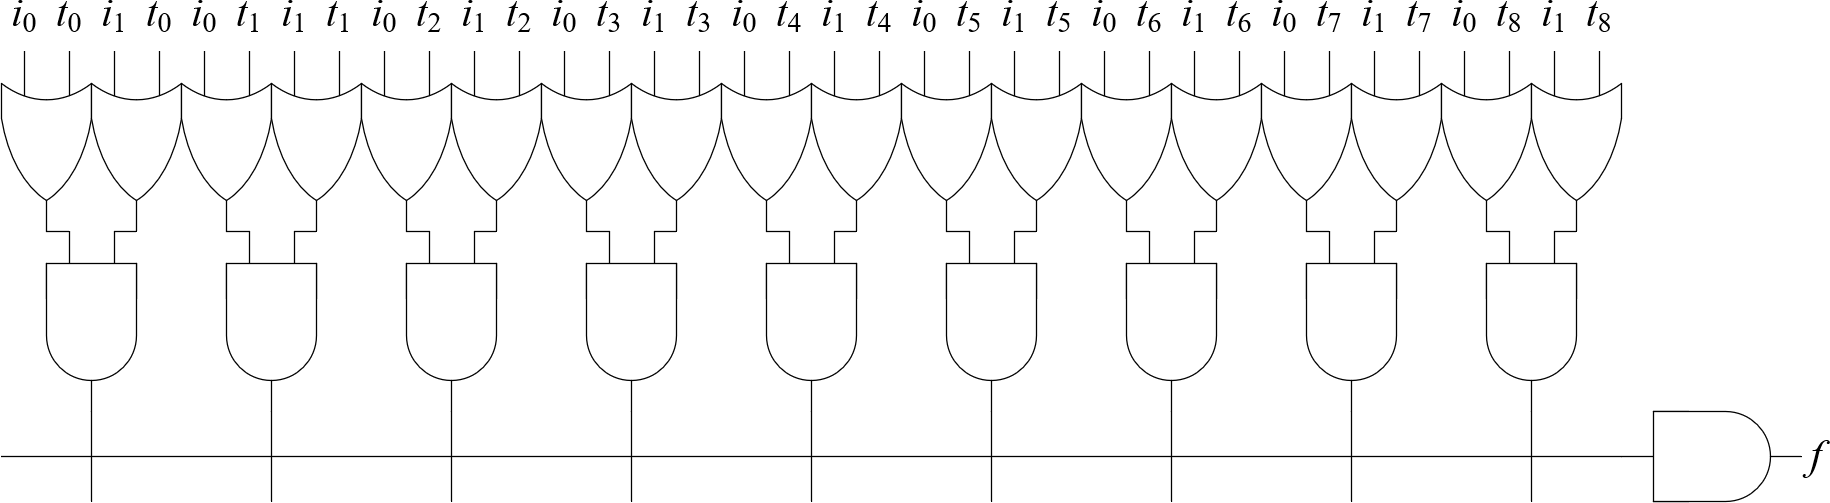
\includegraphics[width=\textwidth]{Product of sums attack}
\caption{Stealthy and malicious circuit with $n=9$ trigger inputs.}
\label{Product of sums attack}
\end{figure}

How to integrate this attack into HT2? First, since in the original HT2 in Figure \ref{HT2-1}, \verb|HT_normal_out| comes directly out of registers in \verb|final_round|, to evade UCI detection, I have to move one operation of \verb|final_round| after the last stage of the registers: AddRoundKey. This operation is shown in Figure \ref{AddRoundKey}.

\begin{figure}[htp] \centering
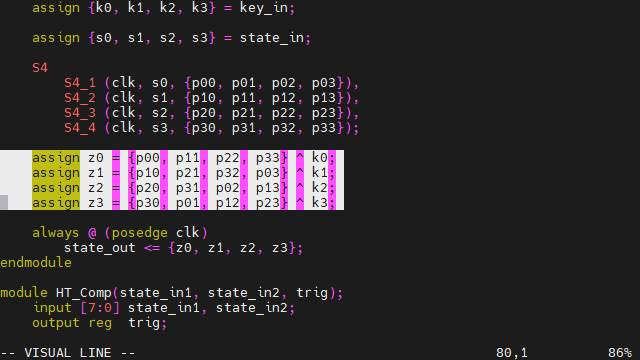
\includegraphics[width=\textwidth]{AddRoundKey}
\caption{AddRoundKey in \texttt{final\_round}.}
\label{AddRoundKey}
\end{figure}

Then, since the payload sets the output to 0 instead of 1, to simplify the integration, I shall change the last AND gate to NAND. As a result, the normal functionality of Figure \ref{Product of sums attack} becomes $f=i_0\text{ NAND }i_1$, and the payload sets $f=0$.

However, AddRoundKey is an XOR operation, not a NAND. How to integrate the normal functionality of XOR into the attack? One possible way is to rewrite XOR as an OAI circuit, as shown in Figure \ref{XOR_OAI}.

\begin{figure}[htp] \centering
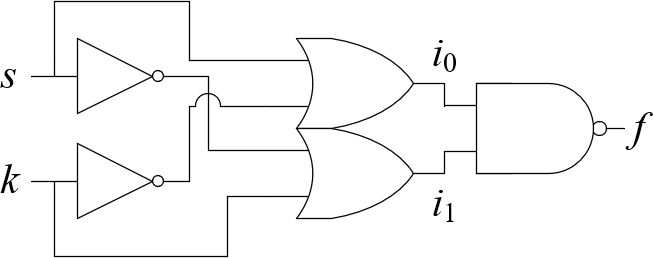
\includegraphics[width=0.5\textwidth]{XOR_OAI}
\caption{The XOR circuit in the OR-AND-INVERT form.}
\label{XOR_OAI}
\end{figure}

Now, since the last gate of Figure \ref{XOR_OAI} is a NAND gate, I can replace that gate with the attack circuit in Figure \ref{improvedHT2} to complete the attack. Finally, the resulting code coverage is shown in Figure \ref{improveHT1}.

\begin{figure}[htp] \centering
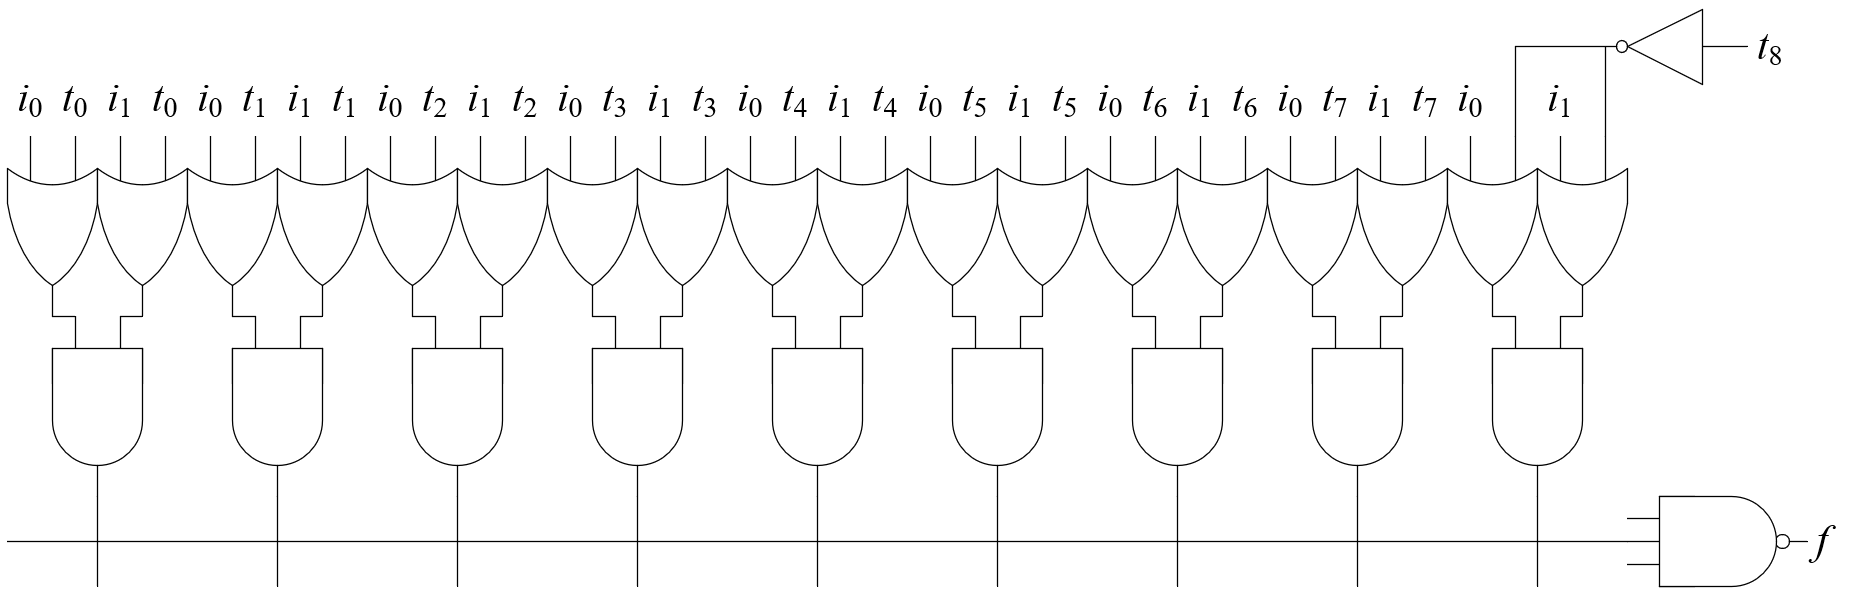
\includegraphics[width=\textwidth]{improvedHT2}
\caption{The attack in Figure \ref{Product of sums attack} adapted into HT2. $i_x$ refers to Figure \ref{XOR_OAI} and $t_x$ refers to \texttt{HT\_cond[x]}. Note that the trigger condition is \texttt{HT\_cond == 9'b0\_1111\_1111}.}
\label{improvedHT2}
\end{figure}

\begin{figure}[htp] \centering
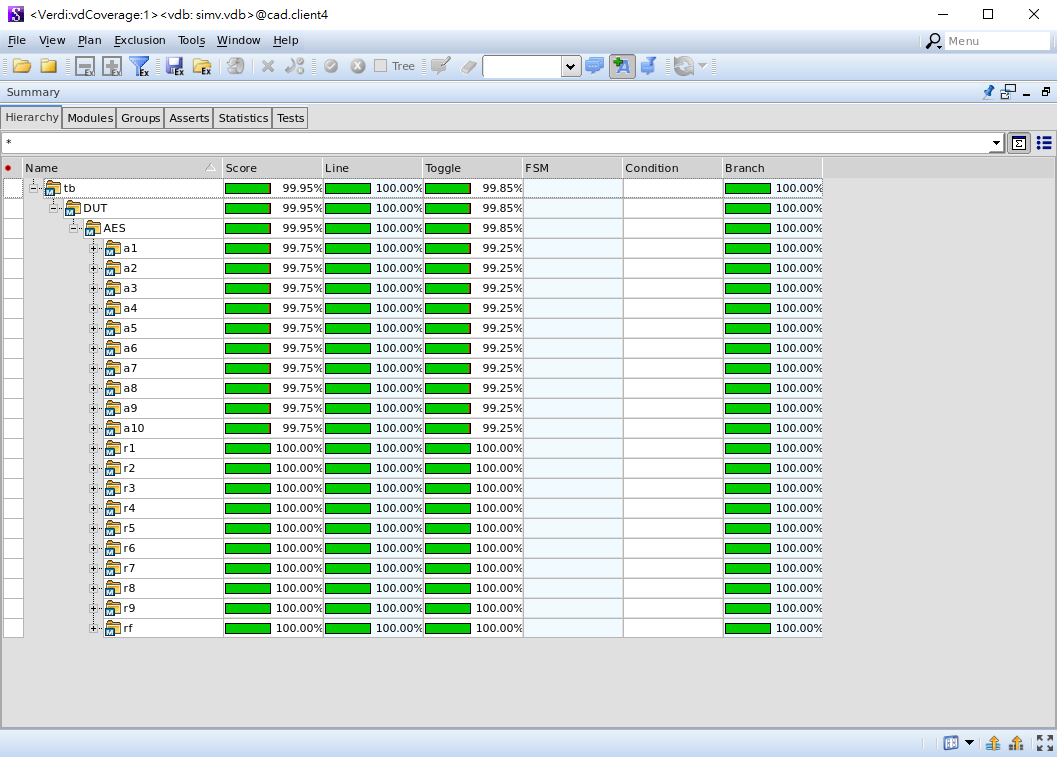
\includegraphics[width=\textwidth]{improveHT2}
\caption{The code coverage of \texttt{HT2/improveHT}.}
\label{improveHT2}
\end{figure}

\subsection{HT3}

Since the code coverage of HT3 is already perfect and I classified HT3 as a side-channel Trojan, it might be reasonable to reference a paper related to side-channel Trojans. The one I referenced is MOLES. \cite{5361303} In addition to the side-channel strategies, what MOLES does is to employ an LFSR to "encrypt" the leaked key, as shown in Figure \ref{MOLES_LFSR}. In my implementation, one such LFSR is (re)used to encrypt every byte of the key (notice that only 8 bits in the LFSR is used to encrypt the key in Figure \ref{MOLES_LFSR}.) I also removed the condition \verb|HT_key == 128'd0|, so an encrypted key is leaked every clock cycle. I didn't remove the reset, however, so that the charges accumulated in the capacitors can also be reset (?)

\begin{figure}[htp] \centering
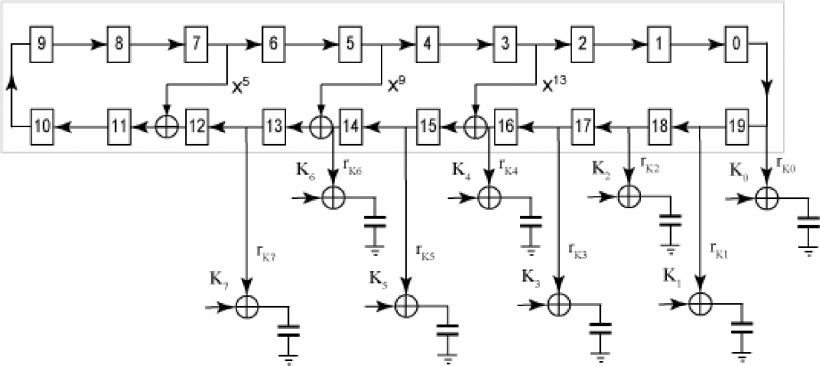
\includegraphics[width=\textwidth]{MOLES_LFSR}
\caption{Figure 2 of \cite{5361303}. My LFSR and the "encrypting" positions are the same as this figure.}
\label{MOLES_LFSR}
\end{figure}

Again, the resulting code coverage is shown in Figure \ref{improveHT3}.

\begin{figure}[htp] \centering
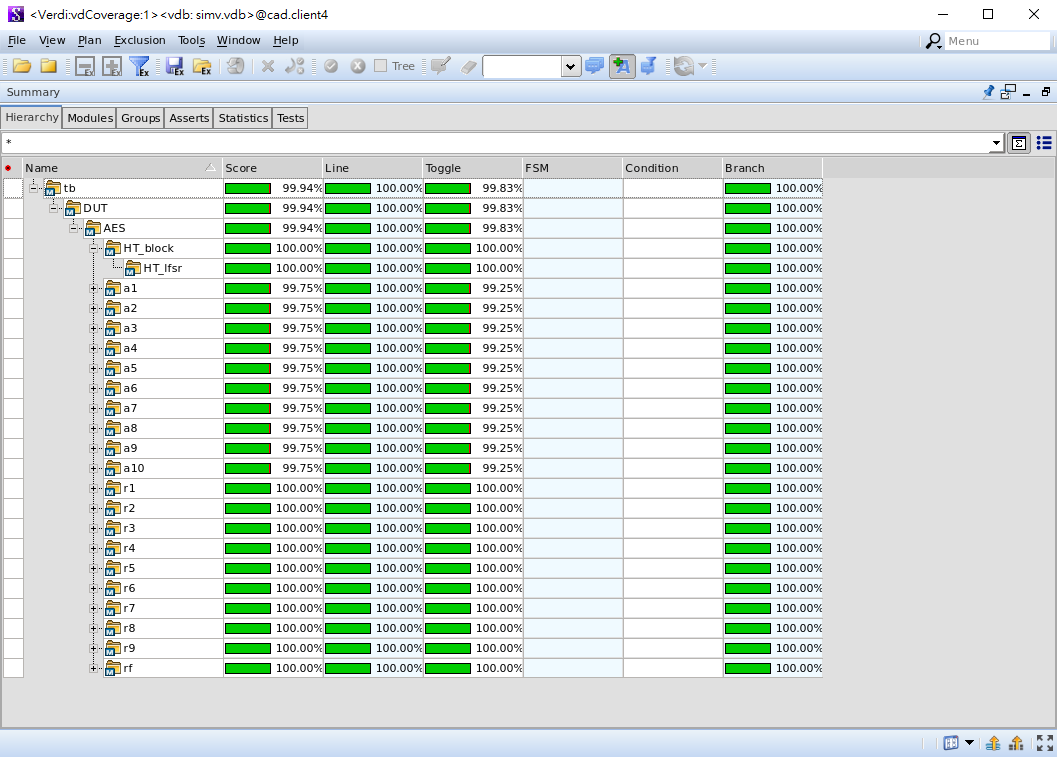
\includegraphics[width=\textwidth]{improveHT3}
\caption{The code coverage of \texttt{HT3/improveHT}.}
\label{improveHT3}
\end{figure}

\section{Difficulties Encountered}

This programming assignment is a huge difficulty spike. First of all, I used to think that the usage of VCS is assumed to be a prerequisite. So, I sought help from my team leader, who took the VLSI course by the same professor last semester. It was not until a few days before the deadline that he revealed that he did not know how to use VCS either. Other issues related to VCS are already mentioned in section 1.

However, the last part of the assignment, namely improving the stealthiness of HTs, turns out to be even more difficult. To the best of my knowledge, there are few papers that target code coverage. So, even if I have a lot of different ideas, it is likely that I cannot find any paper related to my idea(s). Also, \verb|HT_dynamic_key| is just weird at the RTL. I don't really have a good idea on how to improve it. Section 4.3 is my best effort already (and I don't think that is a good one...)

\printbibliography

\end{document}
